\documentclass[12pt]{article}
\usepackage{graphicx}
\begin{document}
\section{Detector Operations}
At the beginning of the quarter, CMS had a successful cosmic ray run with the magnet at 3.8 Tesla in preparation for beam.   This was followed by LHC running with single beams for commission which allowed CMS to use beam halo and splash events to further its commission efforts.    During this period it became apparent that there was contamination in the liquid helium of the CMS magnet.  The decision was taken to turn off the magnet and investigate the source of contamination and replace filters as necessary.   

The investigation of the issues with the magnet�s helium supply continued through the quarter.  At the present time the source of the contamination is not well understood however a detailed analysis showed that it was unlikely that the contamination could reach the magnet itself.  The decision was taken at the end of the quarter to ramp up the magnet and periodically replace filters as necessary.   By July 6 the magnet was again operating at 3.8 Tesla.   

CMS is presently collecting data with LHC collisions at sqrt(s)=13 TeV.  Physics data is being collected and commissioning ongoing while they increase the number of bunches in the beam step-by-step.

\subsection{Milestones and Metrics}
US CMS has developed a set of milestones and metrics for 2015 to measure performance.   At the present time the detector is still being commissioned and so we do not report metrics.   Milestone progress is reported for each subsystem individually below.





\subsection{BRIL}
The main emphasis of the US-CMS effort as part of the BRIL sub-detector group is the pixel 
luminosity telescope (PLT). The detector is installed inside the CMS detector close to the
beam pipe, about 170cm away from the interaction point on either side of it. 
On each side there are 8 3-layer silicon pixel detectors. The detector is kept at -15 degrees
Celsius. The rate of triple coincidences is used to provide luminosity measurements for each
bunch crossing. The framework is in place to continuously publish this information and this
has been done over the last two months. Furthermore, the PLT also monitors the beamspot
online using full pixel detector information that is sampled at a lower rate. Luminosity is 
also calculated from this hit information and using tracking algorithms. 
The PLT has participated in the very first short VdM scan and a first calibration of the 
published luminosity numbers has been done. Online monitoring for all the BRIL sub-systems is 
in place and developed further. The offline analysis code is ready and systematic studies started.
     
One out of 16 telescopes developed a fault after the temperature was raised and reduced for the
barrel pixel detector several times. It is thought that contact problem might have been introduced during
installation that due to temperature changes developed further. This is not expected to
significantly reduce the luminosity precision and for consistent reporting the telescope is 
presently taken out. 

\begin{table}[htdp]
\caption{BRIL Milestones}
\begin{center}
\begin{tabular}{|l|l|r|r|}
\hline
Subsystem&Description&Scheduled&Achieved\\
\hline
BRIL & Hardware installed& Jan & Jan\\
\hline
BRIL& Ready to deliver Lum& March & March \\
\hline
BRIL & Ready to deliver bkg nums& May & May\\
\hline
\end{tabular}
\end{center}
\label{BRILMIlestones}
\end{table}%


\subsection{Tracker}

\subsubsection{Strips}

Using the collisions with no magnetic field, the strips have completed primary timing and bias scans, and identified and found coping mechanisms for problems. We have found that pneumatic control lines in the cooling system can become clogged with ice. The mitigation mechanism is to include a bleed valve that continually flushes the lines. Currently, the correct flow rate for the bleed is being determined. This is important as a loss of cooling in part of the strip detector will effect running. Most of our other operations have been concerned with detector maintenance and learning to operate with the new VME controllers, the new timing system and the upgraded DAQ. 

\subsubsection{Pixels}

Pixels also took advantage of collisions with no field to perform the primary bias and timing scans. The pixels will do a follow-up timing scan with the B field on (the B field effects the cluster size). There have been several issues for pixels with the new DAQ and timing system, and as with the strips, these have been understood and fixed. There is a problem in the BPiX that effects one sector (about 1.6\% of the system). Only part of that sector can hold power when the B field is present. We have tried to include as many modules as possible in the inner barrel layer and all the modules in the outer layer. More testing will be done on the BPiX with the B field returns in July.




\begin{table}[htdp]
\caption{Tracker Milestones}
\begin{center}
\begin{tabular}{|l|l|r|r|}
\hline
Subsystem&Description&Scheduled&Achieved\\

Tracker & Installation and checkout& & Achieved\\
\hline
Tracker & Tracker operate -15C & & Achieved\\
\hline
Tracker & Pixel operate -10C & & Achieved\\
\hline
Tracker& Ready for proton beams& March & March\\
\hline
\end{tabular}
\end{center}
\label{TrackerMilestones}
\end{table}%


\subsection{ECAL}
ECAL is running smoothly with first collisions following the consolidation and development work performed during LS1. Commissioning with beam commenced in April with beam splash events, for which ECAL provided the reference trigger signal. The readout timing of EB, EE and ES was checked and adjusted using beam splashes and first collisions events. These data were also used to and adjust the timing alignment of the EB and EE trigger primitives and to commission the electron/photon Level-1 trigger path.

\begin{figure}[htbp]
\begin{center}   
	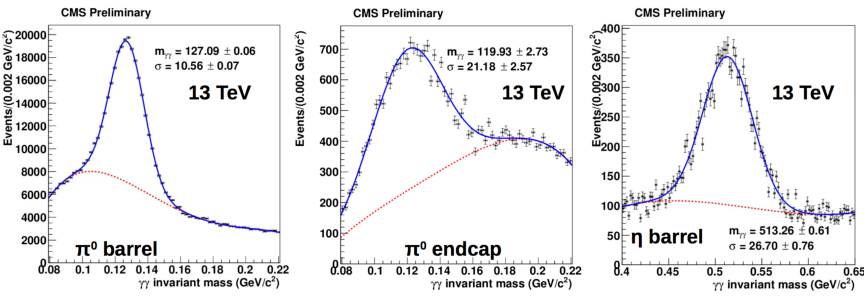
\includegraphics[width=.75\textwidth]{Pi0.pdf}   
\end{center}
\label{fig:Pi0}
\caption{Reconstructed $\pi^{0}$ and $\eta$ peaks from 13 TeV pp collisions} 
\end{figure}

We have successfully exercised the $\pi^0 /\eta$ reconstruction code for calibration using first 13 TeV collisions data obtained from the minimum bias dataset. Figure \ref{fig:Pi0} shows clear $\pi^0 $ and $\eta$ peaks observed in both the barrel and the endcaps. These data are being used for first signal intercalibration and will also be used to verify the timing intercalibration constants.

The upgrade of the barrel ECAL high voltage system has now been completed. The mainframes have been replaced with more efficient CAEN models. A new calibration system has been installed as shown in Fig. 3. The HV system supplies the avalanche photodiode detectors used to readout the crystals. The gain is very sensitive to the HV and hence the calibration is important. The new system will enable an improved calibration to be performed in 24 hours versus the previous 2 weeks that were required. 

\begin{table}[htdp]
\caption{ECAL Milestones}
\begin{center}
\begin{tabular}{|l|l|r|r|}
\hline
Subsystem&Description&Scheduled&Achieved\\
\hline
ECAL & Finish HV Install& Feb & May\\
\hline
ECAL & Baseline levels zero suppression& March & March \\
\hline
ECAL & Complete install HV calib system & April &May\\
\hline
ECAL & Selective readout& June & delayed\\
\hline
ECAL & Trigger thresholds & June & delayed\\
\hline
ECAL & Zero suppression thresholds & June & delayed \\
\hline
\end{tabular}
\end{center}
\label{ECALMilestones}
\end{table}%

The milestones that were dune in June have been slightly delayed by the reported problems with the magnet.   All these features have been tuned as far as possible without the magnetic field and will be finalized with magnetic field data.



\subsection{HCAL}
The HF has participated fully in collisions  so far with the upgraded $\mu$TCA backend (installed in late 2104)
delivering good quality data. The objective of high reliability physics  running for HF has been basically achieved. 
HF Trigger Primitives to were delivered to the Regional Calorimeter Trigger (RCT).
The Look-Up-Tables (LUTs) were updated for the new PMT gains.
The remaining single split  crate with VME legacy electronics has 
been a useful tool in verifying the functionality of the new backend. 
The work done on the HF backend proved extremely useful in getting the $\mu$TCA 
backend for HBHE up and running in  record time during this current LHC 
technical stop.

\begin{table}[htdp]
\caption{HCAL Milestones}
\begin{center}
\begin{tabular}{|l|l|r|r|}
\hline
Subsystem&Description&Scheduled&Achieved\\
\hline
HCAL& Fully functional HCAL in CRAFT runs & March & March\\
\hline
HCAL& prepared to do HF Phase scan & &\\
&and $\phi$ symmetry calibration analysis& May& May\\
\hline
HCAL&New HBHE backend operating in& &\\
& parallel with legacy system& July &\\
\hline
\end{tabular}
\end{center}
\label{HCALMilestones}
\end{table}%


\subsection{EMU}
The CSC system participated all of the start-up and tuning
runs, including beam splash, beam halo, 900 GeV collisions, and
finally stable collisions at 13 TeV.
The beam runs were used to first check the timing of the CSC
trigger and data paths. The initial timing settings for the new
and refurbished chambers were derived earlier this year from
cosmic ray running. They were found to be close to optimal.
The first runs with collisions were reconstructed and examined
in detail. Generally the CSC data looked very good with much
lower fraction of missing channels than in Run 1.
 \begin{table}[htdp]
\caption{EMU Milestones}
\begin{center}
\begin{tabular}{|l|l|r|r|}
\hline
Subsystem&Description&Scheduled&Achieved\\
EMU& CSC ready for collisions& May & April \\
\hline
EMU& Calibration for HLT and & &\\
& Offline included in DB & July & \\
\hline
EMU & Fine timing adjustments & & \\
&with collision data completed & July & \\
\hline
\end{tabular}
\end{center}
\label{EMUMilestones}
\end{table}%


\subsection{DAQ}

Installation of new DAQ including new HLT nodes was completed and routinely used in data taking with Beam and Cosmic runs.  Hardware to read Trigger and HCAL uTCA feds were installed and SLinkExpress (fiber data links that connect the uTCA feds toe DAQ readout modules) are operating at 4 Gbps. Trigger and HCAL sub-systems are using them using central DAQ and MiniDAQ.  

Using emulated data, the Event Building performance has already reached the Run I design performance (100 kHz L1 accept rate for 1 MB Events) with full DAQ chain - event building, high level trigger  (HLT) processing (actually emulated as sleep) and collecting HLT selected event in to single streams ready to be send to tier 0, in emulation runs. This needs to be confirmed  with real detector data with full the HLT menu but for that we need to wait for the LHC luminosity to increase. 

\begin{table}[h]
\caption{DAQ Milestones}
\begin{center}
\begin{tabular}{|l|l|r|r|}
\hline
Subsystem&Description&Scheduled&Achieved\\
\hline
DAQ& Hardware Installation of DAQ2& & \\
& with new HLT nodes complete& April & April \\
\hline
DAQ& Complete DAQ2 is operational && \\
&for collisions& July &   May\\
\hline
DAQ&$\mu$TCA DAQ link commissioned & & \\
&for new trigger and HCAL FEDs& July &  June \\
\hline
DAQ&DAQ2 with Run I design performance & September & \\
\hline
\end{tabular}
\end{center}
\label{DAQMilestones}
\end{table}%


\subsection{Trigger}
During this quarter the US groups continued their work on the regional calorimeter (RCT) and the endcap muon triggers.  In both significant progress was made timing in the various elements of the triggers using beam collisions.  
\subsubsection{Regional Calorimeter Trigger}
During the last three months, the configuration and monitoring of the RCT with the optical RCT Summary Card  was done with the Trigger Supervisor.  Several iterations of the sequence were necessary to insure link stability before the GCT main crate configuration, and now it is very reliable. The RCT with oRSCs participated in the first collisions of LHC Run 2, and the oRSCs have operated without issues since then.
\subsubsection{Endcap Muon Trigger}
The Endcap Muon Trigger was successfully used to trigger on the first stable beam collisions at 13 TeV! The system wass successfully timed-in for halo muons and for first collisions. The DT/CSC data exchange is also timed-in for the most part, but possible fine-tuning of the DT data from the outer wheels may be required once we collect data with the CMS magnet on.

\begin{table}[h]
\caption{Trigger Milestones}
\begin{center}
\begin{tabular}{|l|l|r|r|}
\hline
Subsystem&Description&Scheduled&Achieved\\
\hline
TRIG&Legacy RCT ready for physics&June &June\\
\hline
TRIG&MPC ready for physics&June &June\\
\hline
TRIG&CSCTF Ready for physics&June & June\\
\hline
TRIG& Stage-1 Layer-1 calorimeter trigger&&\\
& ready for physics &September&\\
\hline
\end{tabular}
\end{center}
\label{TriggerMilestones}
\end{table}%



\end{document}

